\documentclass[12pt, a4paper]{article}

% Packages dependencies
\usepackage[brazil]{babel}
\usepackage[top=3cm, bottom=2cm, left=3cm, right=3cm]{geometry}
\usepackage{graphicx}
\usepackage{float}
\usepackage{minted}
\usepackage{xcolor}
\usepackage[labelformat=empty]{caption}
\usepackage{amsmath}
\usepackage{amssymb}
\usepackage{multicol}
\usepackage{indentfirst}
\usepackage{hyperref}
% \usepackage{fontspec}
\usepackage{titlesec}
\usepackage{enumitem}
\usepackage[most]{tcolorbox}
\usepackage{cleveref}
\hypersetup{
    colorlinks=true,
    urlcolor=blue,
    linkcolor=blue
}
% \setmainfont{ARIAL.TTF}[
%   ItalicFont = ARIALI.TTF,
%   BoldFont = ARIALBD.TTF,
%   BoldItalicFont = ARIALBI.TTF,
%   Path = ./fontes/
% ]
\setmonofont{JetBrains Mono}[
Scale=MatchLowercase,
Ligatures=TeX,
Contextuals=Alternate
]
\newtcolorbox{mybox}[2][]{breakable,sharp corners, skin=enhancedmiddle jigsaw,parbox=false,
boxrule=0mm,leftrule=2mm,boxsep=0mm,arc=0mm,outer arc=0mm,attach title to upper,
after title={.\ }, coltitle=black,colback=gray!10,colframe=black, title={#2},
fonttitle=\bfseries,#1}
\renewcommand*\contentsname{SUMÁRIO}

\graphicspath{{images/}}

%Preamble
\date{\today}

%Variable Student Name
\newcommand\studentName{Matheus de Freitas Weber}
\newcommand\studentTwoName{Gabriel Berwanger Silveira}
\newcommand\studentThreeName{Aluno 3}
\newcommand\studentFourName{Aluno 4}

%Variable Course Name
\newcommand\courseName{Circuitos microprocessados}

%Variable Article Name
\newcommand\titleName{Exercício - Aula 02}

%Variable Article SubName
\newcommand\subTitleName{Álgebra booleana com arduino}

%Variable Teacher Name
\newcommand\teacherName{Jean Schmith}

%Body
\begin{document}

% -- Unisinos title -- %
\begin{center}
	\MakeUppercase{\textbf{Universidade do Vale do Rio dos Sinos (Unisinos)}}

	% -- Course Name -- %
	\MakeUppercase{\textbf{Graduação em Engenharia de controle e automação}} \\[16ex]


	% -- Student Name -- %
	\MakeUppercase{\textbf{\studentName}}
	\\
	\MakeUppercase{\textbf{\studentTwoName}}
	\\[16ex]

	% -- Work Title -- %
	\MakeUppercase{\textbf{\titleName}}

	\textbf{\subTitleName}

	\vfill

	\textbf{São Leopoldo}

	\textbf{2025}

	\thispagestyle{empty}
\end{center}
\newpage

% -- Capa -- %
\begin{center}
	% -- Capa -- %
	\vspace*{28ex}
	\MakeUppercase{\studentName}
	\\
	\MakeUppercase{\studentTwoName}
	\vspace*{16ex}

	\MakeUppercase{\textbf{\titleName}}

	\textbf{\subTitleName}

	\vspace*{8ex}

	% -- Description of the work -- %
	\hfill\begin{minipage}{0.5\linewidth}
		Trabalho apresentado para a matéria {\courseName} pelo Curso de Engenharia de Controle e Automação e Engenharia da Computação da Universidade do Vale do Sinos (UNISINOS), ministrada pelo Prof.\teacherName.
	\end{minipage}
	\vfill

	\textbf{São Leopoldo}

	\textbf{2025}

\end{center}
\thispagestyle{empty}
\setcounter{page}{1}
\newpage

% -- Summary -- %
\begin{center}
	\tableofcontents
\end{center}
\thispagestyle{empty}
\newpage

% -- Introduction -- %
\section{Introdução}
\subsection{Objetivo}
O objetivo deste trabalho é apresentar o uso de arduino para a implementação de circuitos lógicos
e a manipulação de sinais digitais, utilizando a álgebra booleana como base para a construção dos circuitos.

\subsection{Questões a serem respondidas}
\begin{enumerate}[label=(\alph*)]
	\item $A \cdot B$
	\item $A + B$
	\item $A + BC$
	\item $AB + \overline{AC}$
\end{enumerate}

\subsection{Implementação Simulada}
Para a simulação dos circuitos lógicos, utilizamos o software Tinkercad, que permite a criação de circuitos eletrônicos virtuais e a programação de microcontroladores como o Arduino.
\newpage

% -- Teorical foundation -- %
\section{Resolução}
\subsection{
	Questão (a): $A \cdot B$
}
\begin{minted}[frame=single, fontsize=\footnotesize]{c}
#define A 8
#define B 9
#define C 10
#define Out 13

bool A = false;
bool B = false;
bool C = false;

void setup() {
  pinMode(A, INPUT);
  pinMode(B, INPUT);
  pinMode(C, INPUT);
  pinMode(Out, OUTPUT);
  Serial.begin(9600);
}

void loop() {
  A = !digitalRead(8);
  B = !digitalRead(9);
  C = !digitalRead(10);

  if (A && B) {
      digitalWrite(Out, HIGH);
    } else {
      digitalWrite(Out, LOW);
    }
  }
\end{minted}

\newpage
\subsection{
	Questão (b): $A + B$
}
\begin{minted}[frame=single, fontsize=\footnotesize]{c}
#define A 8
#define B 9
#define C 10
#define Out 13

bool A = false;
bool B = false;
bool C = false;

void setup() {
  pinMode(A, INPUT);
  pinMode(B, INPUT);
  pinMode(C, INPUT);
  pinMode(Out, OUTPUT);
  Serial.begin(9600);
}

void loop() {
  A = !digitalRead(8);
  B = !digitalRead(9);
  C = !digitalRead(10);

  if (A || B) {
      digitalWrite(Out, HIGH);
    } else {
      digitalWrite(Out, LOW);
    }
  }
\end{minted}

\newpage
\subsection{
	Questão (c): $A + BC$
}
\begin{minted}[frame=single, fontsize=\footnotesize]{c}
#define A 8
#define B 9
#define C 10
#define Out 13

bool A = false;
bool B = false;
bool C = false;

void setup() {
  pinMode(A, INPUT);
  pinMode(B, INPUT);
  pinMode(C, INPUT);
  pinMode(Out, OUTPUT);
  Serial.begin(9600);
}

void loop() {
  A = !digitalRead(8);
  B = !digitalRead(9);
  C = !digitalRead(10);

  if (A + (B && C)) {
      digitalWrite(Out, HIGH);
    } else {
      digitalWrite(Out, LOW);
    }
  }
\end{minted}

\newpage
\subsection{
	Questão (d): $AB + \overline{AC}$
}
\begin{minted}[frame=single, fontsize=\footnotesize]{c}
#define A 8
#define B 9
#define C 10
#define Out 13

bool A = false;
bool B = false;
bool C = false;

void setup() {
  pinMode(A, INPUT);
  pinMode(B, INPUT);
  pinMode(C, INPUT);
  pinMode(Out, OUTPUT);
  Serial.begin(9600);
}

void loop() {
  A = !digitalRead(8);
  B = !digitalRead(9);
  C = !digitalRead(10);

  if ((A && B) || !(A && C)) {
      digitalWrite(Out, HIGH);
    } else {
      digitalWrite(Out, LOW);
    }
  }
\end{minted}

\newpage
\subsection{TinkedCAD}
\subsubsection*{Código completo}
\begin{mybox}{Selecionando a questão}
	Para selecionar a questão, basta descomentar a linha correspondente no código acima.
\end{mybox}
\begin{minted}[frame=single, fontsize=\footnotesize]{c}
#define a
//#define b
//#define c
//#define d

#define pinoA 8
#define pinoB 9
#define pinoC 10
#define pinoSaida 13

bool A = false;
bool B = false;
bool C = false;

void setup(){
	pinMode(pinoA, INPUT);
	pinMode(pinoB, INPUT);
	pinMode(pinoC, INPUT);

 	pinMode(pinoSaida, OUTPUT);
  	
  	Serial.begin(9600);

}

void loop(){
  
  A = !digitalRead(pinoA);
  B = !digitalRead(pinoB);
  C = !digitalRead(pinoC);

  
    #ifdef a
      if(A && B){
        digitalWrite(pinoSaida, HIGH);
      } else {
        digitalWrite(pinoSaida, LOW);
      }
    #endif

    #ifdef b
  	  if(A || B){
        digitalWrite(pinoSaida, HIGH);
      } else {
        digitalWrite(pinoSaida, LOW);
      }
    #endif

    #ifdef c
      if(A || (B && C)){
        digitalWrite(pinoSaida, HIGH);
      } else {
        digitalWrite(pinoSaida, LOW);
      }
    #endif

    #ifdef d
      if((A && B) || (!A && C)){
        digitalWrite(pinoSaida, HIGH);
      } else {
        digitalWrite(pinoSaida, LOW);
      }
    #endif
}
\end{minted}

\subsubsection*{Circuito}
\begin{mybox}{Acionamento dos pinos}
	Os pinos 8, 9 e 10 são acionados por botões 1, 2 e 3 respectivamente que, quando acionados, conectam o pino ao GND (nível lógico baixo). O pino 13 está conectado a um LED que indica o estado da saída do circuito lógico.
\end{mybox}
\begin{center}
	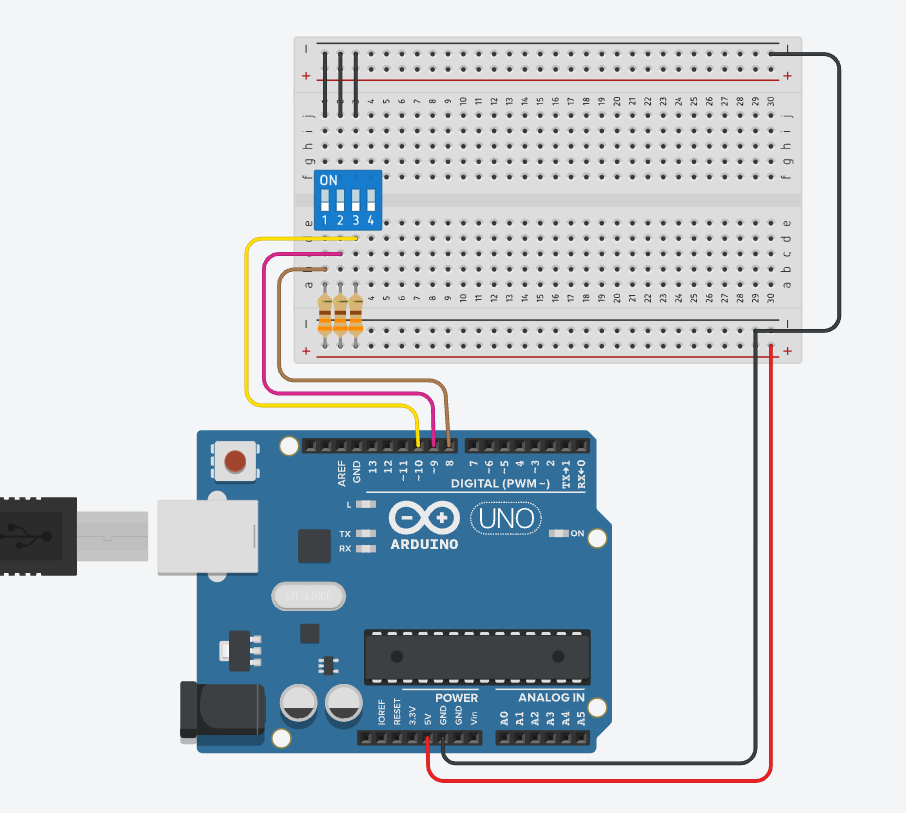
\includegraphics[width=0.8\textwidth]{arduino.png}
\end{center}
\subsubsection*{Link}
\href{https://www.tinkercad.com/things/hr4xBZ8MEj2/editel?returnTo=%2Fdashboard%2Fdesigns%2Fcircuits&sharecode=fPopBI4bYJNTvhWgjXuX53nz_p1ZSa5-tAANBvz1cPw}{Clique aqui} para acessar o circuito no Tinkercad.

\newpage
% -- Conclusion -- %
\begin{center}
	\section{Conclusão}
\end{center}

Neste trabalho, foi possível explorar a álgebra booleana e sua aplicação em circuitos lógicos utilizando o Arduino. Através da simulação no Tinkercad, foi possível verificar o funcionamento dos circuitos lógicos implementados, bem como compreender a lógica por trás de cada operação booleana. A prática com o Arduino proporcionou uma melhor compreensão dos conceitos teóricos e sua aplicação prática, além de desenvolver habilidades de programação e eletrônica.

\end{document}
